\documentclass{article}
\usepackage[utf8]{inputenc}
\usepackage[letterpaper,margin=1in,footskip=0.25in]{geometry}
\usepackage{graphicx}

\title{Explicación Diagramas: Bases de Datos\\
Práctica 02}
\author{Jorge Francisco Cortés López\\
Diego Estrada Mejia}
\date{Agosto 2019}

\begin{document}

\maketitle

\section{Restricciones del modelo entidad relación.}
Empezaremos describiendo las entidades que se utilizaron para la realización del diagrama y su razón del porqué se hicieron de esa manera.\\
\textbf{Cliente:} Esta entidad es de las más obvias, ya que la necesitamos para poder tener un lugar donde almacenar los datos de cada cliente, en esta tenemos varios atributos que nos serán de utilidad para poder tener un modelo bien definido sobre cada cliente como: nombre, dirección y fecha de nacimiento. Los atributos multivaluados que tenemos son el correo electrónico, ya que así está especificado en el problema y también el teléfono. Luego por decisión del modelo, necesitamos una llave que nos ayude a identificar más rápido a cada cliente, por lo que creamos un atributo llamado \textbf{idCliente}. Finalmente como atributo generado tendremos el número de viajes que podremos calcular fácilmente con la información que esté relacionada cuando un cliente reserve un viaje.\\
\textbf{Tarjeta de Cliente Frecuente:} Como se especifica en el problema cada cliente deberá tener una tarjeta de cliente frecuente en la cuál debemos de saber cuántos puntos tenemos en relación con el número de viajes que un cliente haya tenido y además irse actualizando conforme el cliente los use, por lo que tendremos un atributo generado llamado: puntos, luego una llave que estará asociada a cada cliente llamada: \textbf{idTarjeta}. Se decidió que cada tarjeta tenga una llave única ya que sólo un cliente puede tener una tarjeta y una tarjeta estará asociada a un sólo cliente. De aquí que exista la relación \textbf{tener} uno a uno respecto a \textbf{Cliente} y \textbf{Tarjeta de cliente frecuente} y además la relación con respecto a \textbf{Tener} será total, ya que no puede existir una tarjeta sin que exista un cliente.\\
\textbf{Viaje:} Luego de aquí un cliente puede \textbf{reservar} un viaje, por lo que lo más lógico es que exista una relación entre el cliente y la entidad viaje para poder saber las características de el viaje de cada cliente. Un cliente puede realizar múltiples viajes, sin embargo un viaje puede ser reservado sólo por un cliente por lo que la relación \textbf{Reservar} será varios a uno. Un viaje puede tener atributos de interés general como lo son: origen, destino, el tiempo del viaje, el costo y tipo de viaje (privado o compartido). Luego como atributo multivaluado puede ser la forma de pago, ya que un cliente puede pagar, por ejemplo, con la tarjeta de cliente frecuente y pagar lo restante en efectivo. Como atributos generados podemos tener las placas del automovil, que como veremos después será un atributo (llave) de la entidad automovil; el nombre del conductor que puede ser generado de la entidad \textbf{conductor} que veremos más adelante. Y finalmente como llave para identificar cada viaje que un cliente realiza con mayor facilidad.\\
\textbf{Conductor:} Como es lógico, en cada viaje participaran dos entidades principales, el cliente y el conductor. El conductor es similar al cliente en cuanto a sus atributos, como: nombre completo, dirección, fecha de nacimiento. De igual manera multivaluados como teléfono y correo electrónico. El número de viajes que como mencionamos estará relacionado un conductor a si acepta un viaje, y además un conductor puede realizar múltiples viajes, sin embargo un viaje puede ser aceptado sólo por un conductor, por lo que la relación \textbf{Aceptar} será de varios a uno. También nos es importante asociar una llave a cada conductor para identificarlo más fácilmente por lo que tendremos un atributo \textbf{idConductor}.\\
\textbf{Relaciones Reservar y Aceptar:} Como se puede ver ambas relaciones tienen un atributo que es \textbf{Ubicación}, esto debido a que la especificación del problema menciona que es importante saber en donde se encuentra el cliente y el conductor para poder asociarlos de una manera más eficiente con respecto al viaje que el cliente va a reservar.\\
\textbf{Automóvil:} Finalmente tenemos la entidad automovil que es donde se realizará el viaje, un automóvil puede tener como atributos: marca, submarca, color, precio de factura, submarca y año. Como atributos generados podemos tener la categoría, ya que como está en la especificación del problema un automóvil puede caer en una categoría dependiendo del precio de factura, luego el número de asientos puede ser generado dependiendo a su categoría también debido a las restricciones de cada categoría. Entre la entidad automóvil y conductor existe la relación \textbf{Manejar} que es el automóvil asociado a cada conductor, entonces puede suceder que un automóvil cambie de conductor o que un conductor cambie de automóvil, por lo que la relación deberá ser uno a uno, esto es evidente, ya que un automóvil no puede ser manejado por dos conductores al mismo tiempo ni un conductor manejar dos automóviles al mismo tiempo. Como llave podríamos agregar un nuevo atributo, sin embargo cada automóvil tiene asociado una placa por lo que lo más lógico es utilizar ese atributo como llave.\\
A continuación podemos ver el diagrama ER:

\begin{center}
    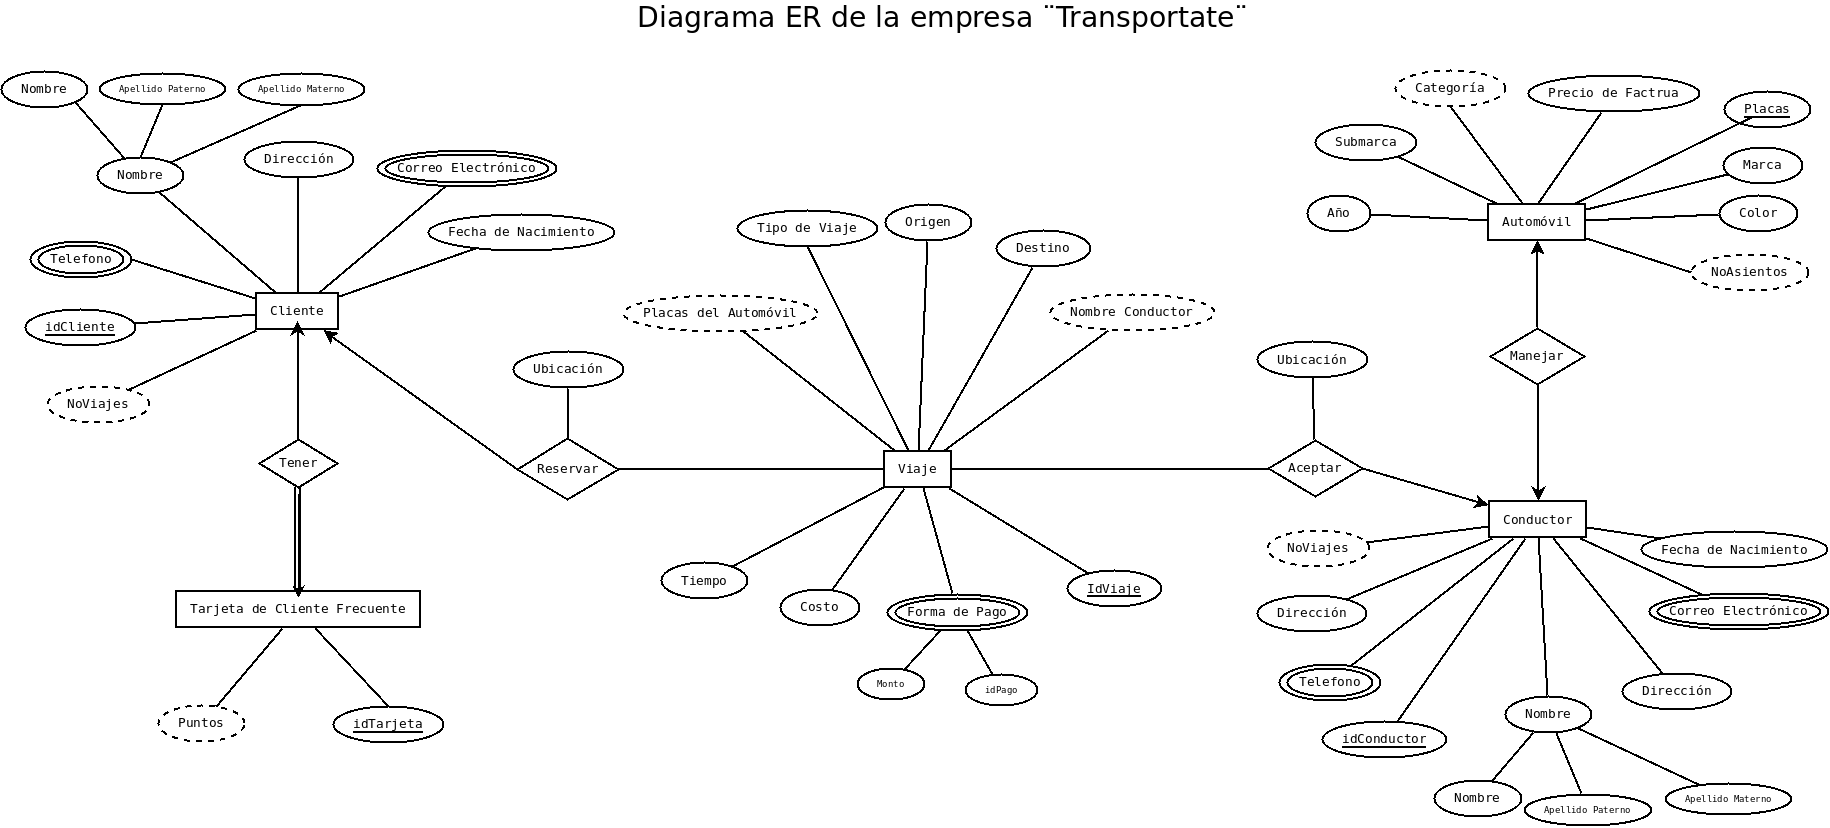
\includegraphics[width=165mm]{Diagrama.png}
\end{center}

\begin{center}
    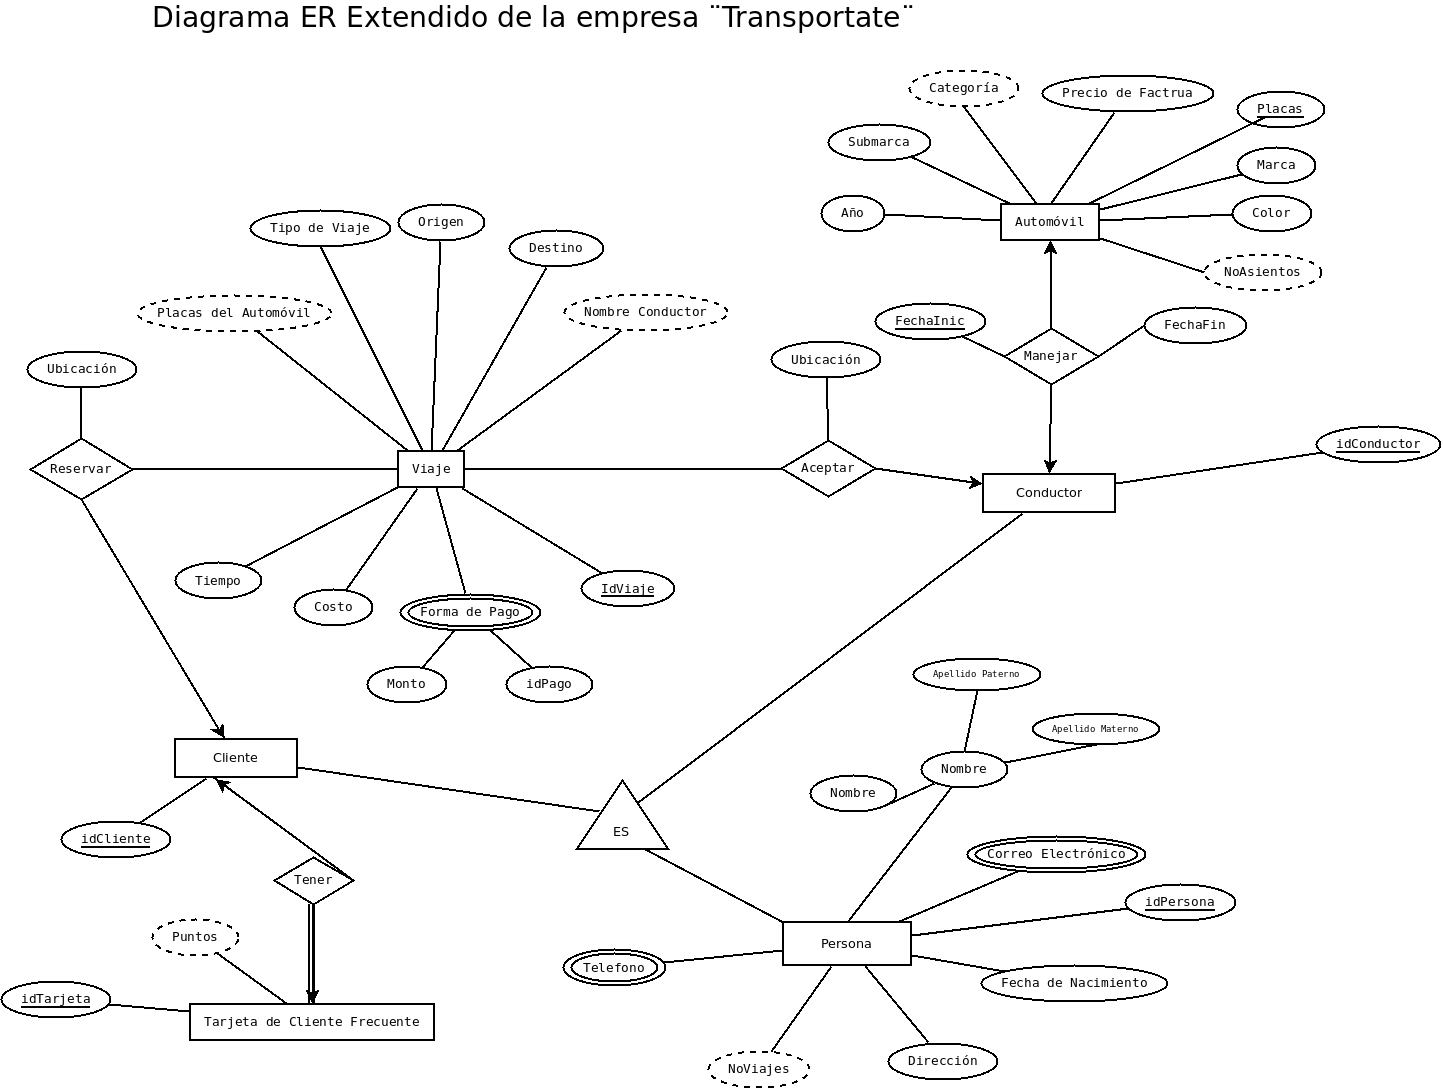
\includegraphics[width=165mm]{DiagramaExtendido.png}
\end{center}

\end{document}
